\section{Palavras, subpalavras e ordem}
\label{sec:bpe}
\subsection{Comparação pareada de tokenizadores}
Mantivemos arquitetura, dimensões, dropout, inicialização numérica,
minibatches e orçamento. Treinamos três CNNs com BPE e reutilizamos três
checkpoints por palavras. Ambas as receitas usam Adam a 0,001, escolhido
antes no estudo por palavras. Cada execução seleciona a época na validação.
O pareamento controla os pesos iniciais como matrizes numéricas. As linhas
de embedding correspondem a unidades distintas em cada vocabulário.

\begin{tabularx}{\linewidth}{@{}Xrrrrr@{}}
\toprule
\tabelahead{Tokenizer} & \tabelahead{Acurácia} & \tabelahead{F1 macro} &
\tabelahead{CE} & \tabelahead{UNK} & \tabelahead{Tokens médios}\\
\midrule
\LinhasBPE
\bottomrule
\end{tabularx}
\legendinha{Tabela 7. Nova auditoria interna, com 2.048 resenhas. Métricas
médias de três sementes. UNK conta a proporção de tokens desconhecidos.}

\vspace{2mm}
\begin{minipage}[c]{.51\linewidth}
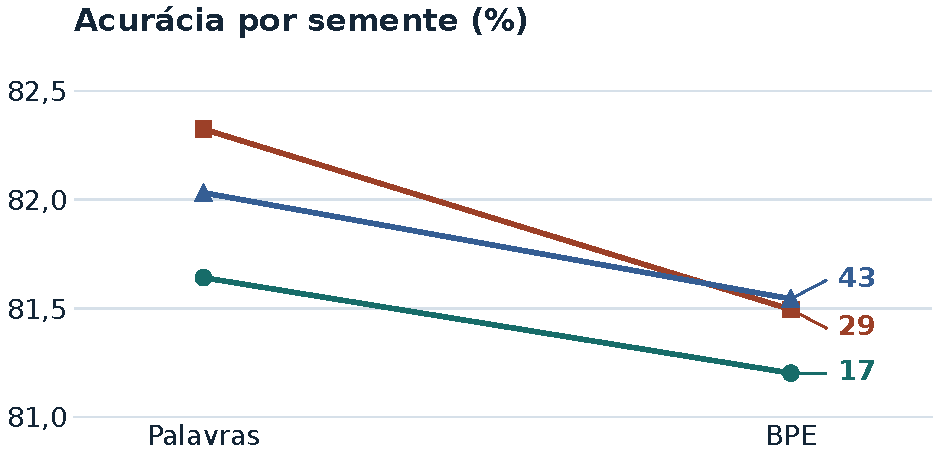
\includegraphics[width=\linewidth]{figuras/bpe_pareado.pdf}
\end{minipage}\hfill
\begin{minipage}[c]{.45\linewidth}
A diferença média é de \(-0,59\) ponto percentual para BPE. A cobertura
melhorou e a sequência ficou mais longa. Um filtro de cinco tokens pode
cobrir menos palavras, o que muda o contexto que ele observa. Esta
comparação estima o desempenho sob a taxa herdada e as larguras fixas.
\end{minipage}
\legendinha{Figura 3. Cada linha une a mesma semente sob as duas tokenizações.
Eixo vertical ampliado. \fonte{results/bpe/audit_metrics.json}{Métricas por execução}.}

\subsection{Pares sintéticos com a mesma contagem de palavras}
Escrevemos quatro pares antes da inferência e congelamos a lista em
\texttt{seminario/casos.json}. Verificamos a igualdade dos unigramas e
calculamos janelas de IDs de larguras 3, 4 e 5 com cada tokenizer.
Os seis checkpoints escolhidos no protocolo BPE foram executados em CPU.
Os números abaixo são médias de escores positivos antes de calibração.

\begin{tabularx}{\linewidth}{@{}Xrrrrl@{}}
\toprule
 & \multicolumn{2}{c}{\tabelahead{Palavras}} & \multicolumn{2}{c}{\tabelahead{BPE}} & \\
\cmidrule(lr){2-3}\cmidrule(lr){4-5}
\tabelahead{Par} & \tabelahead{A} & \tabelahead{B} & \tabelahead{A} & \tabelahead{B} &
\tabelahead{Trocas P/B}\\
\midrule
\LinhasPares
\bottomrule
\end{tabularx}
\legendinha{Tabela 8. Trocas de classe entre A e B em três sementes para palavras
e BPE. Aspectos e troca de blocos têm leitura mista. Os escores por semente,
IDs, janelas e hashes estão em \texttt{dados/pares\_resultados.json}.}

Em \textit{The movie is good, not bad}, a troca de \textit{good} e
\textit{bad} reduz o escore positivo médio nos dois tokenizadores.
Na semente 17, a própria frase A recebe \NegacaoPalavrasA{} com palavras
e \NegacaoBPEA{} com BPE. O limiar 0,5 dá classes diferentes para o mesmo
texto nas duas receitas treinadas.
No par da Seção~\ref{sec:ordem}, a troca muda a classe em todas as sementes
e inverte a leitura esperada. A Seção~\ref{sec:falhas} explica como o
controle com janelas iguais separa a reação local de um limite estrutural.
